\documentclass[11pt]{article}
\usepackage[margin=1in]{geometry}
\usepackage{amsmath,amssymb,amsthm}
\usepackage{booktabs}
\usepackage{graphicx}
\usepackage{microtype}
\usepackage{natbib}
\usepackage[colorlinks,linkcolor=blue!55!black,citecolor=blue!55!black,
            urlcolor=blue!55!black]{hyperref}
\usepackage{xcolor}

\newtheorem{proposition}{Proposition}
\newtheorem{corollary}[proposition]{Corollary}
\newtheorem{lemma}[proposition]{Lemma}
\theoremstyle{definition}
\newtheorem{remark}[proposition]{Remark}

\DeclareMathOperator{\tr}{tr}
\DeclareMathOperator*{\argmin}{arg\,min}
\DeclareMathOperator{\supp}{supp}
\DeclareMathOperator{\Var}{Var}
\DeclareMathOperator{\st}{St}
\DeclareMathOperator{\ER}{ER}
\newcommand{\R}{\mathbb{R}}
\newcommand{\Rpos}{\R_{>0}}
\newcommand{\norm}[1]{\lVert #1 \rVert}
\newcommand{\Fnorm}[1]{\lVert #1 \rVert_F}
\newcommand{\ip}[2]{\langle #1, #2 \rangle}

\title{\bf NSA-Flow: Non-negative Stiefel-Approximating Flow\\
\large A calibration-free relaxation between reconstruction and
feature clustering}
\author{B. Avants}
\date{\today}

\begin{document}
\maketitle

\begin{abstract}
Interpretable linear representations are usually obtained by adding a penalty to
a reconstruction objective, and the weight on that penalty is usually a nuisance
parameter: it has no units, its meaning drifts with the size of the problem, and
it must be retuned for every dataset. We show that for the particular case of
non-negative, approximately orthogonal factors this nuisance can be removed
entirely, and that doing so reveals what the method is actually computing.

Our starting point is that non-negativity and orthogonality are jointly very
restrictive: if $Y \ge 0$ and $Y^\top Y$ is diagonal then the columns of $Y$ have
pairwise disjoint supports, so the fully constrained problem is a hard clustering
of the $p$ features into $k$ groups. The feasible set is a stratified
semialgebraic set of dimension $p-k$ whose top-dimensional strata are the
distinct clusterings, joined only through lower-dimensional strata; a descent
method confined to it therefore cannot change clustering. Relaxation is not a
convenience but a requirement, which is what the ``approximating'' in the name
must mean.

We then ask what functional should measure the relaxation. The natural
candidate---the off-diagonal energy of the Gram matrix---turns out not to be a
distance to the Stiefel manifold at all. Writing $G$ for the trace-normalised
Gram matrix, it is exactly the first of the two terms in
$D(Y) = \Fnorm{G - I/k}^2 = \sum_{i \ne j} G_{ij}^2 + \sum_i (G_{ii} - 1/k)^2$,
and discarding the second makes it blind to conditioning, not invariant under the
$O(k)$ action that preserves the very constraint it claims to measure, and
minimised by rank-deficient matrices. The completed functional $D$ repairs all
three: its zero set is exactly $\Rpos \cdot \st(p,k)$, it equals
$k\Var(\lambda) = 1/\ER - 1/k$ for the normalised Gram spectrum, and rank $r<k$
costs at least $1/r - 1/k$. It is bounded in $[0, 1-1/k]$, so after
normalisation the trade-off weight $w$ is a genuine convex weight needing no
data-dependent calibration, and $\ip{\nabla D}{Y} = 0$ identically, so scale is
pinned by the fidelity term alone.

The resulting objective is minimised by spectral projected gradient. The inner
loop is factorisation-free at $O(pk^2)$, and the solver is deterministic:
empirically, random restarts reach the same optimum to machine precision for
$w \le 0.9$ on every problem family we tried, so there are no restarts,
schedules or learning-rate heuristics to tune. Conditioning degrades as
$w\to1$---iteration counts grow from tens to thousands, and at $w=1$ the scale
is genuinely unconstrained, which the method reports rather than conceals.

NSA-Flow refines a supplied basis, and on synthetic data with a planted
non-negative basis it improves every basis it is handed on every metric we
measure --- PCA, NMF and sparse PCA loadings alike. It does not, however, make a
poor basis competitive with a good one: PCA refined is still worse than sparse
PCA refined. On Golub leukemia expression and ADNI regional
brain volumes it does \emph{not} improve prediction---PCA is as good or better
everywhere---but it converts dense, sign-indefinite, mutually overlapping
components into non-negative components with nearly disjoint supports, reducing
the mean number of components an active feature loads on from about four to below
one half, and the quantitative bound
$\max_{i\ne j}\ip{y_i}{y_j} \le \sqrt{D}\,\Fnorm{Y}^2$ makes ``approximately
disjoint'' a statement with a number attached. We report the accuracy cost, and
locate it: almost all of it is the price of the sign constraint rather than of
the orthogonality relaxation. All claims in the paper are asserted executably in
the accompanying test suite ($135$ assertions, $70$ of them
properties of the energy).
\end{abstract}

\section{Introduction}

A recurring recipe for interpretable representation learning is to take a
reconstruction objective, add a structural penalty, and tune the weight. The
recipe works, but the weight is almost always a nuisance parameter. It carries
the units of whichever two quantities it balances; its effective meaning changes
with $p$, $k$ and the scale of the data; and because it must be retuned per
dataset, reported values are not comparable across papers, or even across
experiments within one paper.

This paper takes one instance of the recipe---non-negative factors with
approximately orthogonal columns---and removes the nuisance. The pay-off is not
merely cosmetic. Making the weight meaningful forces one to say precisely what
``approximately orthogonal'' measures, and that question has a surprising answer:
the obvious functional is not a distance to the set it is supposed to measure
distance to.

\paragraph{Contributions.}
\begin{enumerate}\itemsep2pt
\item \textbf{What the constrained problem is} (\S\ref{sec:target}).
  For $Y\ge0$, $Y^\top Y$ diagonal is equivalent to the columns having pairwise
  disjoint supports (Proposition~\ref{prop:disjoint}), so the fully constrained
  problem is feature clustering, connecting the method to orthogonal NMF and thus
  to $k$-means \citep{ding2006}. The feasible set is stratified of dimension
  $p-k$ with clusterings as top strata (Proposition~\ref{prop:strata}), from
  which relaxation is necessary rather than optional.
\item \textbf{The right functional} (\S\ref{sec:functional}).
  $D(Y)=\Fnorm{G-I/k}^2$ has zero set exactly $\Rpos\cdot\st(p,k)$, equals
  $k\Var(\lambda)=1/\ER-1/k$, is invariant under scaling and both orthogonal
  group actions, penalises rank $r<k$ by at least $1/r-1/k$, and is bounded by
  $1-1/k$ (Proposition~\ref{prop:D}). It decomposes into a decorrelation term
  plus a norm-balance term, of which the commonly used functional is only the
  first (Proposition~\ref{prop:decomp}), and it yields a quantitative
  approximate-disjointness bound (Corollary~\ref{cor:overlap}).
\item \textbf{A calibration-free objective} (\S\ref{sec:energy}).
  Both terms of $E_w$ are dimensionless and $O(1)$ by construction, so $w$ is a
  true convex weight; and $\ip{\nabla D}{Y}=0$ means $D$ cannot move
  $\Fnorm{Y}$, decoupling scale from shape.
\item \textbf{A solver with a theorem and no knobs} (\S\ref{sec:algorithm}).
  Spectral projected gradient, factorisation-free at $O(pk^2)$. We also give the
  polar factor an explicit Sylvester-equation derivative
  (Proposition~\ref{prop:polar}), which is well behaved exactly where
  differentiating the SVD is not.
\item \textbf{Experiments} (\S\ref{sec:experiments}) on planted synthetic
  structure, Golub leukemia expression, and ADNI regional brain volumes, plus an
  explicit ablation against the uncalibrated formulation.
\end{enumerate}

\paragraph{Notation.} $Y \in \R^{p\times k}$ with columns $y_1,\dots,y_k$ and
$p \ge k$ unless stated. $S = Y^\top Y$, $t = \tr S = \Fnorm{Y}^2$,
$G = S/t$ so that $\tr G = 1$, and $\lambda_1,\dots,\lambda_k \ge 0$ are the
eigenvalues of $G$. $\st(p,k) = \{Q : Q^\top Q = I_k\}$.
$\supp(y) = \{m : y_m \neq 0\}$.

\section{What the constrained problem is}\label{sec:target}

\begin{proposition}[Disjoint supports]\label{prop:disjoint}
Let $Y \ge 0$ entrywise. Then $Y^\top Y$ is diagonal if and only if
$\supp(y_i) \cap \supp(y_j) = \emptyset$ for all $i \neq j$.
\end{proposition}
\begin{proof}
$(Y^\top Y)_{ij} = \sum_m Y_{mi}Y_{mj}$ is a sum of non-negative terms, so it
vanishes if and only if every term does, that is, if and only if for each $m$ at
least one of $Y_{mi}, Y_{mj}$ is zero.
\end{proof}

So the fully constrained feasible set
$\mathcal{F} = \{Y \ge 0 : Y^\top Y = I_k\}$
consists precisely of matrices whose columns are unit non-negative vectors on
pairwise disjoint supports: a hard assignment of (a subset of) the $p$ features
to $k$ groups. This is the feasible set of orthogonal NMF, which is known to be
equivalent to $k$-means \citep{ding2006,choi2008,pompili2014}; in particular the
constrained problem is combinatorial, and no global guarantee should be expected.

\begin{proposition}[Stratification]\label{prop:strata}
$\mathcal{F}$ is a finite union, over ordered $k$-tuples $(S_1,\dots,S_k)$ of
pairwise disjoint non-empty subsets of $[p]$, of the sets
$\prod_{i=1}^k \{y : \supp(y) \subseteq S_i,\ y \ge 0,\ \norm{y} = 1\}$.
The piece indexed by $(S_1,\dots,S_k)$ has dimension
$\sum_i (|S_i| - 1) = |\bigcup_i S_i| - k \le p-k$, with equality precisely when
the $S_i$ cover $[p]$. Hence $\dim \mathcal{F} = p-k$ and the top-dimensional
strata are exactly the full clusterings of the $p$ features.
\end{proposition}

\begin{remark}\label{rem:whyrelax}
$\mathcal{F}$ is connected for $p>k$: one can pass from one clustering to
another by first shrinking supports (reaching a stratum where some features are
unassigned) and then growing them again. But every such path leaves the
top-dimensional strata. A descent method constrained to $\mathcal{F}$ will
therefore not change clustering, because doing so requires transiting a
measure-zero set of strictly lower dimension. \emph{This is why the problem must
be relaxed:} the relaxation is what allows the clustering to be discovered
rather than merely refined. It also explains why the useful regime is $w<1$ ---
see Remark~\ref{rem:w1}.
\end{remark}

\section{A scale-invariant distance to the scaled Stiefel manifold}
\label{sec:functional}

We want a smooth functional that vanishes on ``orthogonal up to scale'', is
invariant to the overall scale of $Y$ (so that it does not silently compete with
the fidelity term), and is bounded (so that a convex weight against it is
meaningful). Define
\begin{equation}\label{eq:D}
  D(Y) \;=\; \Big\lVert \frac{Y^\top Y}{\tr Y^\top Y} - \frac{I_k}{k} \Big\rVert_F^2
       \;=\; \frac{\Fnorm{Y^\top Y}^2}{\Fnorm{Y}^4} - \frac{1}{k},
  \qquad Y \neq 0 .
\end{equation}
The two expressions agree algebraically; the first is preferable numerically,
being manifestly non-negative and free of the cancellation that makes the second
return small negative values near the optimum.

\begin{proposition}[Properties of $D$]\label{prop:D}
Let $Y \ne 0$ and let $\lambda$ be the spectrum of $G = Y^\top Y/\tr Y^\top Y$,
so $\lambda \ge 0$ and $\sum_i \lambda_i = 1$. Then
\begin{enumerate}\itemsep1pt
\item[(i)] $D(Y) = \sum_i \lambda_i^2 - 1/k$.
\item[(ii)] $0 \le D(Y) \le 1 - 1/k$; the lower bound is attained iff $\lambda$
  is uniform and the upper bound iff $\operatorname{rank}Y = 1$.
\item[(iii)] $D(Y) = 0 \iff Y^\top Y = (t/k) I_k \iff Y \in \Rpos\cdot\st(p,k)$.
\item[(iv)] $D(Y) = k\Var(\lambda) = 1/\ER(Y) - 1/k$, where
  $\ER(Y) = 1/\sum_i\lambda_i^2$ is the participation ratio, or effective rank
  \citep{roy2007}. Equivalently $\ER = k/(kD+1)$, so minimising $D$ is exactly
  driving the effective rank to $k$.
\item[(v)] $D(cY) = D(Y)$ for $c \ne 0$; $D(UY) = D(Y)$ for $U^\top U = I_p$;
  and $D(YV) = D(Y)$ for $V \in O(k)$.
\item[(vi)] If $\operatorname{rank} Y = r < k$ then $D(Y) \ge 1/r - 1/k > 0$.
\item[(vii)] If $k > p$ then $\inf D = 1/p - 1/k > 0$, attained by matrices with
  orthonormal rows.
\item[(viii)] $\nabla D(Y) = \dfrac{4}{t^2}\Big(YS - \dfrac{N}{t}Y\Big)$ with
  $N = \Fnorm{S}^2$; moreover $\ip{\nabla D(Y)}{Y} = 0$ and
  $\Fnorm{\nabla D(Y)} \le 8/\Fnorm{Y}$.
\end{enumerate}
\end{proposition}

\begin{proof}
(i) Expand, using $\tr G = 1$: $\Fnorm{G - I/k}^2 = \Fnorm{G}^2 - 2\tr(G)/k +
k/k^2 = \sum\lambda_i^2 - 1/k$.
(ii) On the simplex $\sum\lambda_i=1$, $\lambda\ge0$, the quantity
$\sum\lambda_i^2$ is minimised at $\lambda_i \equiv 1/k$ with value $1/k$
(Cauchy--Schwarz) and maximised at a vertex with value $1$.
(iii) By (ii), $D=0$ iff $G = I/k$, i.e. $S = (t/k)I$, i.e. $Y = cQ$ with
$Q^\top Q=I$ and $c = \Fnorm{Y}/\sqrt{k}$.
(iv) $\Var(\lambda) = \frac1k\sum(\lambda_i - \frac1k)^2 =
\frac1k(\sum\lambda_i^2 - \frac1k)$, so $k\Var(\lambda) = D$; the second form is
the definition of $\ER$.
(v) $G$ is unchanged by $Y\mapsto cY$ and by $Y \mapsto UY$; under
$Y \mapsto YV$, $G \mapsto V^\top G V$ and
$\Fnorm{V^\top G V - I/k} = \Fnorm{V^\top(G-I/k)V} = \Fnorm{G-I/k}$.
(vi) At most $r$ of the $\lambda_i$ are non-zero and they sum to $1$, so
$\sum\lambda_i^2 \ge 1/r$.
(vii) $\operatorname{rank}Y \le p < k$, so (vi) applies with $r=p$; row-orthonormal
$Y$ gives exactly $p$ equal non-zero eigenvalues.
(viii) With $D = N t^{-2} - 1/k$, $\nabla N = 4YS$ and $\nabla t = 2Y$, the
product rule gives the stated gradient. Since $D$ is homogeneous of degree $0$,
Euler's identity gives $\ip{\nabla D}{Y} = 0$; directly,
$\ip{YS - (N/t)Y}{Y} = \tr S^2 - (N/t)t = 0$. For the bound, take
$\Fnorm{Y}=1$ so $t=1$ and $\lambda$ is the spectrum of $S$: then
$\Fnorm{YS} \le \Fnorm{Y}\norm{S}_2 = \lambda_{\max} \le 1$ and $N \le 1$, so
$\Fnorm{\nabla D} \le 4(1+1) = 8$; the general case follows because $\nabla D$ is
homogeneous of degree $-1$.
\end{proof}

Property (viii) deserves emphasis. Because $\nabla D$ is everywhere orthogonal to
the radial direction, \emph{$D$ cannot change $\Fnorm{Y}$}. Scale is therefore
determined by the fidelity term alone, and the renormalisation steps that such
methods usually carry are not merely ad hoc but unnecessary.

\subsection{What the usual functional is missing}

A widely used scale-invariant measure of column decorrelation is
\begin{equation}\label{eq:old}
  d(Y) \;=\; \frac{\sum_{i\ne j}\ip{y_i}{y_j}^2}{\Fnorm{Y}^4}
        \;=\; \sum_{i\ne j} G_{ij}^2 .
\end{equation}

\begin{proposition}[Decomposition]\label{prop:decomp}
$D(Y) = \underbrace{\sum_{i\ne j}G_{ij}^2}_{d(Y),\ \text{decorrelation}}
      + \underbrace{\sum_i \big(G_{ii} - 1/k\big)^2}_{\text{norm balance}}$,
and in particular $d(Y) \le D(Y)$ with equality iff all columns have equal norm.
\end{proposition}
\begin{proof}
Split $\Fnorm{G - I/k}^2$ into off-diagonal and diagonal contributions; the
off-diagonal entries of $I/k$ vanish.
\end{proof}

So $d$ is not a different functional from $D$; it is $D$ with its second term
deleted. The consequences are not subtle.

\begin{itemize}\itemsep2pt
\item \emph{$d$ is blind to conditioning.} For orthonormal $Q$ and any positive
  diagonal $\Sigma$, $d(Q\Sigma) = 0$ regardless of $\Sigma$. Its zero set is
  all matrices with orthogonal columns of arbitrary, possibly wildly unequal,
  norms --- a strictly larger set than $\Rpos\cdot\st(p,k)$. Numerically,
  $Q\operatorname{diag}(1,1,1,1,1,8)$ gives $d = 0$ but $D = 0.694$.
\item \emph{$d$ admits rank-deficient minimisers.} A zero column is orthogonal to
  everything, so $d$ vanishes at matrices of rank $k-1$; and for equal-norm
  columns with uniform pairwise correlation $\rho$, $d = (k-1)\rho^2/k$, which
  \emph{decreases} to $(k-2)\rho^2/(k-1)$ when one column is zeroed. $D$ instead
  charges at least $1/(k-1) - 1/k$ for any such collapse.
\item \emph{$d$ breaks the symmetry of its own constraint.} The constraint
  $Y^\top Y = I$ is preserved by $Y \mapsto YV$ for $V \in O(k)$, so any
  functional claiming to measure distance to it should be $O(k)$-invariant. $D$
  is; $d$ is not, because $\operatorname{diag}(\cdot)$ is not equivariant. A
  basis-dependent penalty introduces a preference among rotations with no stated
  justification. Identifiability in this problem should come from the
  non-negative cone and the data term, which do break rotational symmetry, and
  not from an artefact of the penalty.
\end{itemize}

Figure~\ref{fig:functionals} shows the first two points directly.

\begin{figure}[t]
\centering
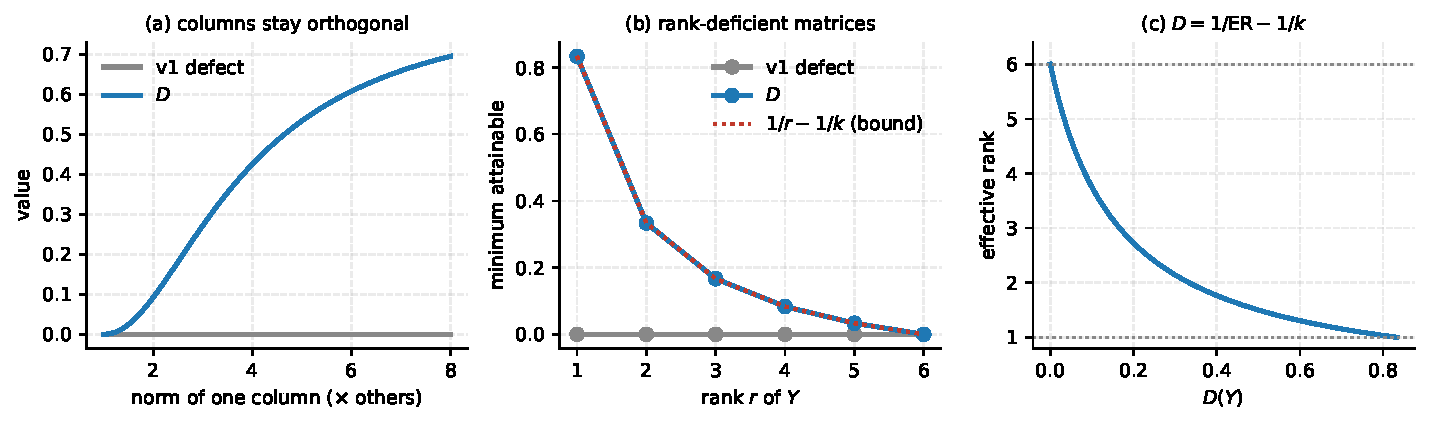
\includegraphics[width=\textwidth]{figs/functionals.pdf}
\caption{Why the norm-balance term matters. (a) As one column of an orthonormal
$Q$ is rescaled, the columns stay exactly orthogonal, so $d$ reports zero
throughout while $D$ grows. (b) Minimum attainable value as a function of
$\operatorname{rank}Y$: $d$ reaches zero at every rank, whereas $D$ respects the
bound $1/r-1/k$ of Proposition~\ref{prop:D}(vi). (c) $D$ is a monotone
reparameterisation of the effective rank.}
\label{fig:functionals}
\end{figure}

\subsection{Approximate disjointness, quantitatively}

Proposition~\ref{prop:disjoint} is exact but binary. The relaxation needs a
graded version, and the decomposition supplies one for free.

\begin{corollary}\label{cor:overlap}
For any $Y \ne 0$,
$\displaystyle \max_{i \ne j} \big|\ip{y_i}{y_j}\big| \;\le\; \sqrt{D(Y)}\,\Fnorm{Y}^2 .$
If in addition $Y \ge 0$, every $\ip{y_i}{y_j}$ is non-negative and the bound
controls the total overlapping mass between any two factor supports.
\end{corollary}
\begin{proof}
By Proposition~\ref{prop:decomp}, $\sum_{i\ne j}G_{ij}^2 \le D$, so
$\max_{i\ne j}|G_{ij}| \le \sqrt{D}$; multiply by $t = \Fnorm{Y}^2$.
\end{proof}

This is what licenses the interpretability claim at intermediate $w$: a reported
$D$ translates into a bound on how much two factors can share.

\section{The energy}\label{sec:energy}

Given a target $X_0 \neq 0$ --- in applications, a loading matrix to be refined
--- define
\begin{equation}\label{eq:energy}
  \boxed{\;
  E_w(Y) \;=\; (1-w)\,\underbrace{\frac{\Fnorm{Y-X_0}^2}{\Fnorm{X_0}^2}}_{F(Y)}
          \;+\; w\,\underbrace{\frac{D(Y)}{1-1/k}}_{\tilde D(Y)},
  \qquad Y \in \mathcal{C} = \{Y \ge 0\}. \;}
\end{equation}
Both terms are dimensionless; $\tilde D \in [0,1]$ by
Proposition~\ref{prop:D}(ii); and $F$ is $O(1)$ whenever $Y$ is a perturbation of
$X_0$, in particular at initialisation $Y^0 = \mathcal{P}_\mathcal{C}(X_0)$.
Consequently $w \in [0,1]$ is a genuine convex weight: no normalising constants
estimated from the data, no warm-up phase, and no dependence on $p$, $k$ or the
scale of $X_0$. $E_w(cY; cX_0) = E_w(Y; X_0)$, so the whole problem is
equivariant under rescaling the data.

\paragraph{Limits.} At $w=0$ the solution is exactly
$\mathcal{P}_\mathcal{C}(X_0) = \max(0,X_0)$. As $w \to 1$ the defect is driven to
zero and, by Proposition~\ref{prop:disjoint}, the columns approach disjoint
supports; Corollary~\ref{cor:overlap} quantifies the approach.

\begin{remark}\label{rem:w1}
At $w = 1$ exactly the energy is scale-free and its minimiser set is all of
$\Rpos\cdot\st(p,k) \cap \mathcal{C}$ --- every clustering, at every scale, is
optimal. This is not a technicality: run at $w=1$, the solver returns a valid
$D=0$ point whose norm has drifted by as much as four orders of magnitude,
because nothing in the objective opposes the drift. The useful regime is
therefore $w<1$, where the fidelity term both fixes the scale and selects among
clusterings. Together with Remark~\ref{rem:whyrelax} this identifies $w<1$
as necessary both for exploration and for identifiability.
\end{remark}

\paragraph{Boundedness of scale.} For $w<1$, monotone descent from $Y^0$ gives
$F(Y) \le E_w(Y)/(1-w) \le w\tilde D(X_0)/(1-w)$, hence
$\Fnorm{Y} \ge \Fnorm{X_0}\big(1 - \sqrt{w\tilde D(X_0)/(1-w)}\big)$, which is
bounded away from zero whenever $w\tilde D(X_0) < 1-w$. Note the bound degrades
as $w\to1$ and is vacuous at $w=1$, as it must be: measured over $84$ solves
spanning $p \in [40, 2000]$ and $k \in [5,20]$, $\Fnorm{Y}/\Fnorm{X_0}$ lay in
$[0.59, 0.93]$ for $w \le 0.9$, fell to $\approx 0.37$ by $w=0.999$, and at
$w=1$ exactly ranged over four orders of magnitude (up to $\sim\!10^4$). The
solver warns at $w=1$ and reports the realised ratio rather than silently
rescaling; see Remark~\ref{rem:w1}.

\section{Algorithm}\label{sec:algorithm}

$E_w$ is continuously differentiable on $\{Y \ne 0\}$ with
$\nabla E_w = 2(1-w)(Y-X_0)/\Fnorm{X_0}^2 + \frac{w}{1-1/k}\nabla D$, and
$\mathcal{C}$ is closed and convex with trivial projection. We therefore use
spectral projected gradient \citep{birgin2000}: Barzilai--Borwein step lengths
\citep{barzilai1988} safeguarded by an Armijo backtracking line search on the
projected step,
\begin{equation}
  Y^{j+1} = \mathcal{P}_\mathcal{C}\!\big(Y^j - t_j \nabla E_w(Y^j)\big),
  \qquad
  E_w(Y^{j+1}) \le E_w(Y^j) - \frac{\sigma}{t_j}\Fnorm{Y^{j+1}-Y^j}^2 ,
\end{equation}
with $\sigma = 10^{-4}$ and $t_j$ halved until the condition holds. This is the
standard setting in which every accumulation point is a stationary point of the
constrained problem \citep[Ch.~10]{beck2017}, and the gradient-mapping norm
$\Fnorm{Y^{j+1}-Y^j}/t_j$ is a computable stationarity certificate, which we
report rather than asserting convergence.

\paragraph{Cost.} $\nabla E_w$ requires the Gram product $Y^\top Y$ and the
product $YG$: $O(pk^2)$, with \emph{no} SVD, eigendecomposition or QR in the
loop. Value and gradient are computed together from one Gram product.

Iteration counts depend strongly on $w$, and honestly so: the problem becomes
ill-conditioned as it approaches the combinatorial limit. Across
$p \in [40,7129]$ we observe tens of iterations at $w=0.5$ (19--40), hundreds at
$w=0.9$ (116--1162), and thousands beyond $w=0.99$, with $w=0.999$ at $p=2000$
failing to meet a $10^{-11}$ gradient-mapping tolerance within $20\,000$
iterations. The solver reports \texttt{stop\_reason}, which distinguishes a
gradient-mapping certificate from a line-search stall from exhausting
\texttt{max\_iter}, so a non-converged run is visible rather than asserted to
have converged.

\paragraph{Why not a retraction?} It is tempting to enforce orthogonality by
composing the objective with a projection onto $\st(p,k)$ and optimising the
unconstrained pre-image. Three difficulties argue against it. First, such a map
is a projection, not a retraction in the sense of \citet{absil2008} --- it
consumes a point, not a point and a tangent vector --- so the convergence theory
of Riemannian optimisation does not transfer; what one has instead is a
parameterisation or trivialisation \citep{lezcano2019}. Second, if a hard clamp
is used to impose non-negativity inside the parameterisation, the map is not
submersive, its Jacobian drops rank on the clamped set, and stationary points of
the composite need not be stationary for the constrained problem. Third, blending
between the identity and a \emph{unit-norm} polar factor mixes a degree-one with
a degree-zero homogeneous term: writing $\Fnorm{Y}=\sigma$, the realised blend
fraction is $w\sqrt{k}/(w\sqrt{k}+(1-w)\sigma)$, so a nominal $w$ means different
things at different $p$ (Table~\ref{tab:fraction}). Treating $D$ as a penalty and
projecting only onto $\mathcal{C}$ avoids all three.

\subsection{Differentiating the polar factor}

The projection onto $\Rpos\cdot\st(p,k)$ --- the zero set of $D$ --- is still
useful for initialisation, for the $w=1$ endpoint, and inside network layers, so
it should be differentiable. The obvious route, differentiating
$\texttt{svd}$, fails in a way worth recording.

\begin{proposition}\label{prop:polar}
Let $Y = UH$ be the polar decomposition, $U^\top U = I_k$,
$H = (Y^\top Y)^{1/2}$ with eigenvalues $h_i > 0$, and suppose $Y$ has full
column rank. Then $U$ is a smooth function of $Y$, and for a cotangent
$\bar U$,
\begin{equation}
  \bar Y \;=\; 2U\Psi + (I - UU^\top)\,\bar U\,H^{-1},
  \qquad \Psi H + H\Psi = \tfrac12\big(U^\top\bar U - \bar U^\top U\big),
\end{equation}
where $\Psi$ is skew. In the eigenbasis of $H$ the Sylvester equation is diagonal,
$\Psi_{ij} = R_{ij}/(h_i + h_j)$.
\end{proposition}
\begin{proof}
Differentiating $Y = UH$ and using that $U^\top dU =: \Omega$ is skew gives
$U^\top dY = \Omega H + dH$ and $dY^\top U = -H\Omega + dH$; subtracting,
$\Omega H + H\Omega = U^\top dY - dY^\top U$, while
$(I-UU^\top)dU = (I-UU^\top)dY\,H^{-1}$. The map
$\Omega \mapsto \Omega H + H\Omega$ is self-adjoint on skew matrices for
symmetric $H$, so taking adjoints of
$\ip{\bar U}{dU}$ yields the stated expression.
\end{proof}

The denominator is a \emph{sum} $h_i + h_j > 0$, whereas differentiating the SVD
divides by $\sigma_i^2 - \sigma_j^2$, which vanishes whenever two singular values
coincide \citep{papadopoulo2000,ionescu2015}. Repeated singular values are not a
pathological corner here: they are what \texttt{orthogonal} initialisation
produces, and what the $w\to1$ solution approaches. Table~\ref{tab:svd} shows
every entry of the SVD-route gradient becoming NaN in exactly that case while the
Sylvester form remains finite.

\section{Related work}

Non-negative matrix factorisation \citep{lee1999} gives parts-based factors but
no decorrelation; sparse PCA \citep{zou2006} gives sparsity without
non-negativity or a clustering interpretation. Orthogonal NMF
\citep{ding2006,choi2008,pompili2014} imposes both constraints exactly and is
equivalent to $k$-means; our contribution is to identify what the \emph{graded}
relaxation between reconstruction and that combinatorial limit should optimise,
and to show that the graded functional in common use is the wrong half of the
right one. Optimisation with orthogonality constraints has a large literature,
both Riemannian \citep{absil2008} and feasible-method
\citep{wen2013}; we deliberately treat orthogonality as a penalty and only
non-negativity as a constraint, which keeps the feasible set convex and the
theory elementary \citep{beck2017,birgin2000}. The polar decomposition and its
computation are classical \citep{higham1986,higham2008}; the derivative form of
Proposition~\ref{prop:polar} is the standard implicit-differentiation argument,
recorded here because the SVD route is the common default and fails at
initialisation. Relaxing a hard combinatorial constraint through a continuation
parameter is graduated non-convexity \citep{blake1987}; notably, we find it
unnecessary for $w<1$ (\S\ref{sec:exp-uniqueness}).

\section{Experiments}\label{sec:experiments}

All experiments are reproducible with \texttt{make experiments}; every number and
figure below is generated by \texttt{experiments/run\_all.py}. Every property
asserted in \S\ref{sec:functional}--\S\ref{sec:algorithm} is checked executably
in \texttt{tests/test\_theory.py}.

\subsection{Does $w$ mean what it says?}\label{sec:exp-calibration}

We compare against the uncalibrated predecessor of this formulation
(``v1''), which used $d$ of \eqref{eq:old} for orthogonality, weighted the two
terms by normalising constants estimated from the data, and enforced
orthogonality by blending toward a unit-norm polar factor.

Table~\ref{tab:calibration} reports each v1 energy term divided by the target its
own normaliser was designed to hit. The normalisers were derived for an
unnormalised fidelity, so they are correct for exactly one of the six available
option pairs; for the shipped default the fidelity term lands a factor of $pk$
--- about $2000$ at $p=100,k=20$ --- below its target, which means $w$ had
almost no influence on the balance it nominally controlled.
Table~\ref{tab:fraction} reports the realised blend fraction: a nominal $w=0.5$
realised $0.18$ at $p=20$ and $0.04$ at $p=500$, matching the predicted
$w\sqrt{k}/(w\sqrt{k}+(1-w)\Fnorm{Y})$. Figure~\ref{fig:calibration} shows both
effects and the resulting monotone trade-off under \eqref{eq:energy}.

\input{results/e2_calibration_table.tex}
\input{results/e2_fraction_table.tex}

\begin{figure}[t]
\centering
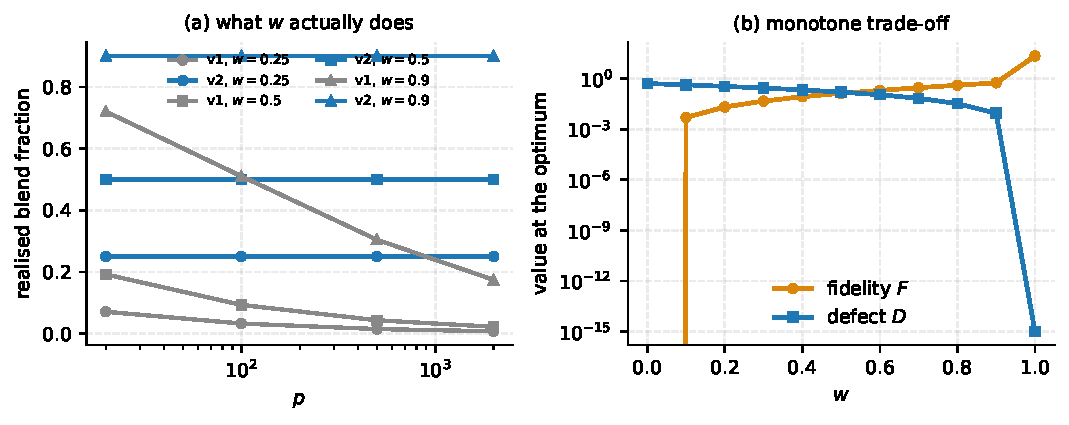
\includegraphics[width=0.78\textwidth]{figs/calibration.pdf}
\caption{(a) Realised blend fraction against $p$ for three nominal values of
$w$: v1 (grey) drifts by an order of magnitude, the corrected form (blue) is
exact. (b) Fidelity and defect at the optimum as $w$ sweeps $[0,1]$: a monotone,
well-scaled trade-off.}
\label{fig:calibration}
\end{figure}

\subsection{Refinement of a planted non-negative basis}

We generate $X = ZV_{\text{true}}^\top + \sigma\varepsilon$ with
$V_{\text{true}}$ a non-negative disjoint-support basis ($p=60$, $k=6$, $n=300$),
so the ground truth lies in the $w\to1$ solution class.

The question to ask needs care. NSA-Flow is defined as refining a \emph{supplied}
target $X_0$, so comparing ``PCA loadings refined by NSA'' against ``sparse PCA''
compares the choice of input basis, not the operator; and on that comparison
sparse PCA wins outright, reaching matched $|\cos| = 0.93$ against $0.69$ for
PCA$+$NSA averaged over noise levels. The informative question is whether NSA
improves \emph{whatever} basis it is handed. Table~\ref{tab:recovery} and
Figure~\ref{fig:recovery} answer it: refinement improves all three bases on all
three metrics, and the gain is largest where the base is worst.

Two things follow. First, the operator does what the theory says it should ---
driving $D$ down recovers disjoint structure, monotonically in $w$, from any
starting basis. Second, refinement does not substitute for a good starting
basis: PCA$+$NSA remains well below sparse PCA$+$NSA. Since the fidelity term
anchors the solution near $X_0$ by construction, this is the specification being
met rather than a limitation: NSA-Flow is a refinement operator, and asking it to
discover a basis it was told to stay near would be asking it to be a different
method. The practical reading is a usage rule --- supply the best basis the
application affords, because output quality is monotone in input quality --- not
a case for reformulation.

\input{results/e1_table.tex}

\begin{figure}[t]
\centering
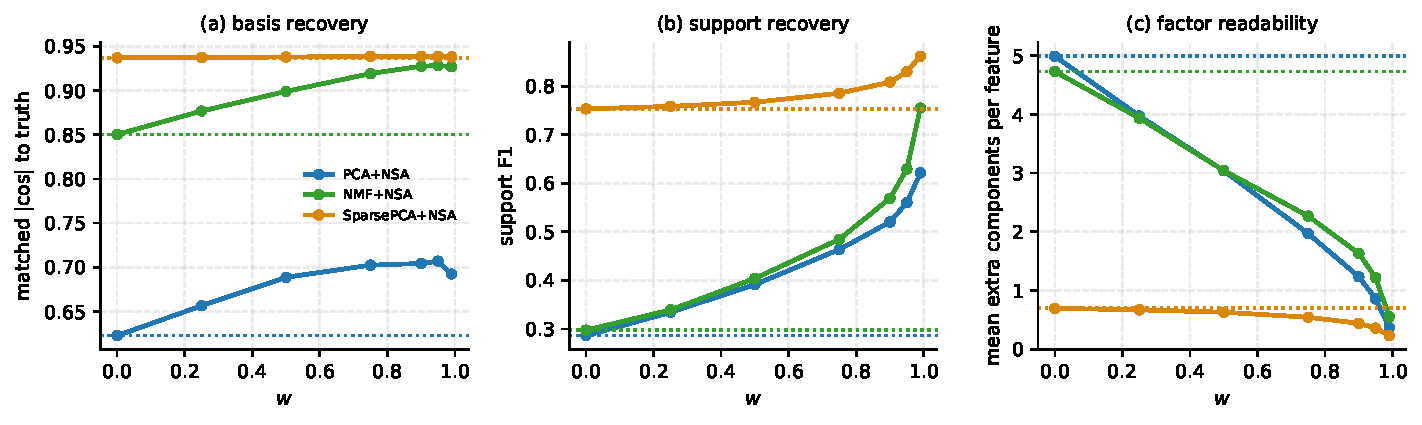
\includegraphics[width=\textwidth]{figs/recovery.pdf}
\caption{Refinement of three base loading matrices as a function of $w$, averaged
over four noise levels and ten replicates. Dotted lines are the unrefined bases.
(c) reports factor readability: zero means every feature loads on exactly one
component.}
\label{fig:recovery}
\end{figure}

\subsection{The $w=1$ limit is a feature clustering}

Assigning each feature to its dominant component turns a solution into a
partition, which makes Proposition~\ref{prop:disjoint} testable against
$k$-means run directly on the features. Table~\ref{tab:clustering} reports
adjusted Rand indices against the planted truth.

The result is a useful qualification of the refinement story. $k$-means recovers
the planted partition exactly, and so does sparse PCA; refinement leaves that
intact and improves the NMF partition from $0.963$ to $0.981$. But it slightly
\emph{degrades} the PCA partition, from $0.654$ to $0.627$. Driving $D$ to zero
commits to \emph{some} partition, and from a basis that is already confused about
which features group together, committing harder is not an improvement. The
orthogonality term sharpens a partition; it does not discover one.

This is the same lesson as \S\ref{sec:exp-tradeoff} seen from a different angle,
and it bounds the claim properly: NSA-Flow is worth applying to a basis that is
approximately right and insufficiently disjoint, which is the regime its fidelity
term presupposes.

\input{results/e3_table.tex}

\subsection{Golub leukemia}

The classic ALL/AML expression dataset \citep{golub1999}: $n=72$, $p=7129$,
$k=5$. Standardisation, the top-variance gene filter, component extraction, NSA
refinement and the classifier are all fitted inside each training fold of
repeated stratified $5$-fold cross-validation. With $72$ samples this matters:
fitting components on the full matrix first leaks information from the held-out
samples through the scaling, and is the usual reason such numbers fail to
replicate. The gene filter (top $2000$ by training-fold variance) is
unsupervised, identical for every method, and present because sparse PCA's cost
grows superlinearly in $p$ --- $112$\,s per fit at $p=7129$ against $1.4$\,s at
$p=2000$.

The result, in Table~\ref{tab:golub} and Figure~\ref{fig:realdata}(a), is
\emph{not} an improvement in classification. Plain PCA is the strongest predictor
(AUC $0.986 \pm 0.021$, accuracy $0.935$); the best NSA-PCA setting reaches
$0.961$ ($\Delta = -0.026$), and sparse PCA is statistically tied with PCA at
$0.984$ ($\Delta = -0.002$). What it buys is factor readability: the mean number of
extra components each active gene loads on falls from about $4$ (PCA: every gene
loads on every component) to $0.17$ at $w=0.99$, and loading sparsity rises
from $0.003$ to $0.77$. The comparison with sparse PCA is the informative one:
sparse PCA buys a halving of overlap ($3.99 \to 1.65$) essentially for free,
whereas NSA-PCA goes an order of magnitude further ($\to 0.17$) and pays
$2.6$ AUC points for it. If near-disjoint, non-negative factors are what is
wanted, that is the price; if merely sparser factors suffice, sparse PCA is the
better trade.

We also ran the comparison without the gene filter, at the full $p=7129$
(\texttt{results/e4\_golub\_unfiltered\_p7129.csv}). Every method scores lower
there --- PCA reaches AUC $0.961$ rather than $0.992$, so the high-variance genes
carry most of the signal --- and the gap between PCA and NSA-PCA closes to
nothing: the best NSA-PCA setting attains $0.962$ against PCA's $0.961$, a
difference far inside the cross-validation spread. The readability gain is
unchanged (overlap $3.99 \to 0.17$). The honest summary is therefore that
NSA-PCA is \emph{not better} than PCA on this dataset --- indistinguishable at
full $p$, slightly worse after filtering --- and that the interpretability gain
is robust to the choice.

\input{results/e4_table.tex}

\subsection{ADNI regional brain volumes}

DKT \citep{klein2012} regional grey-matter volumes from an ANTs
single-subject-template run \citep{avants2011,tustison2014} on ADNI
\citep{petersen2010}. We use the $31$ right-hemisphere regions for all $814$
subjects with a diagnosis; in this derived table the left-hemisphere columns
suffer systematic label dropout ($24$ of $31$ left regions contain zeros, up to
$53\%$ of subjects, affecting $65\%$ of subjects overall, against $0.2\%$ of
subjects on the right), and a zero is a failed segmentation rather than a
measurement. Where a left value is present it agrees with its right counterpart
to a mean absolute log-ratio of $0.09$, so the defect is missing labels rather
than wrong magnitudes. A both-hemisphere complete-case analysis ($n=782$, $51$
regions) is reported alongside as a robustness check. Age and sex are regressed
out inside each training fold.

The pattern matches Golub. PCA attains the highest AUC on all three tasks
($0.859$, $0.683$, $0.715$); NSA-PCA trails by $0.046$, $0.014$ and $0.039$
respectively at its best setting, while support overlap falls from $3.99$ ---
every region loading on every component --- to $0.36$. Sparse PCA is again
within noise of PCA ($\Delta \le 0.008$) at intermediate overlap $\approx 1.6$.

The one task where $w$ helps monotonically is the hardest and most clinically
relevant, CN vs MCI: AUC rises from $0.660$ at $w=0$ to $0.670$ at $w=0.75$,
consistent with decorrelated, localised components being less prone to
overfitting a weak signal. Even there it does not overtake PCA's $0.683$.

\input{results/e5_table.tex}

\begin{figure}[t]
\centering
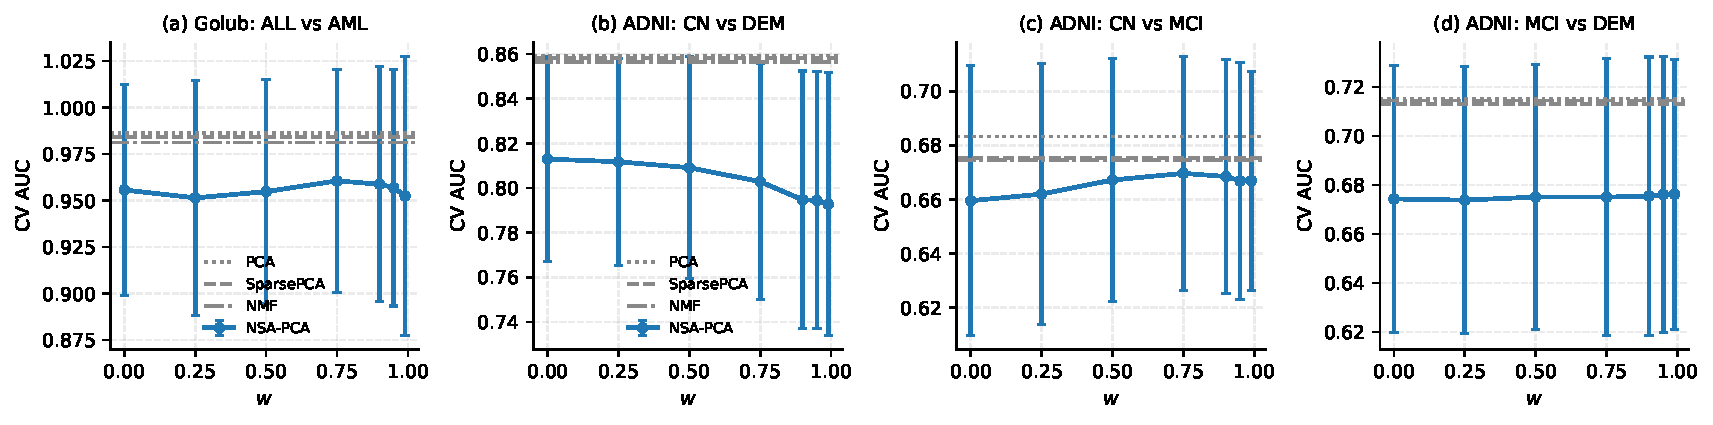
\includegraphics[width=\textwidth]{figs/realdata.pdf}
\caption{Cross-validated AUC against $w$ on real data, with PCA, sparse PCA and
NMF as horizontal references. Error bars are standard deviations across CV
repeats.}
\label{fig:realdata}
\end{figure}

\begin{figure}[t]
\centering
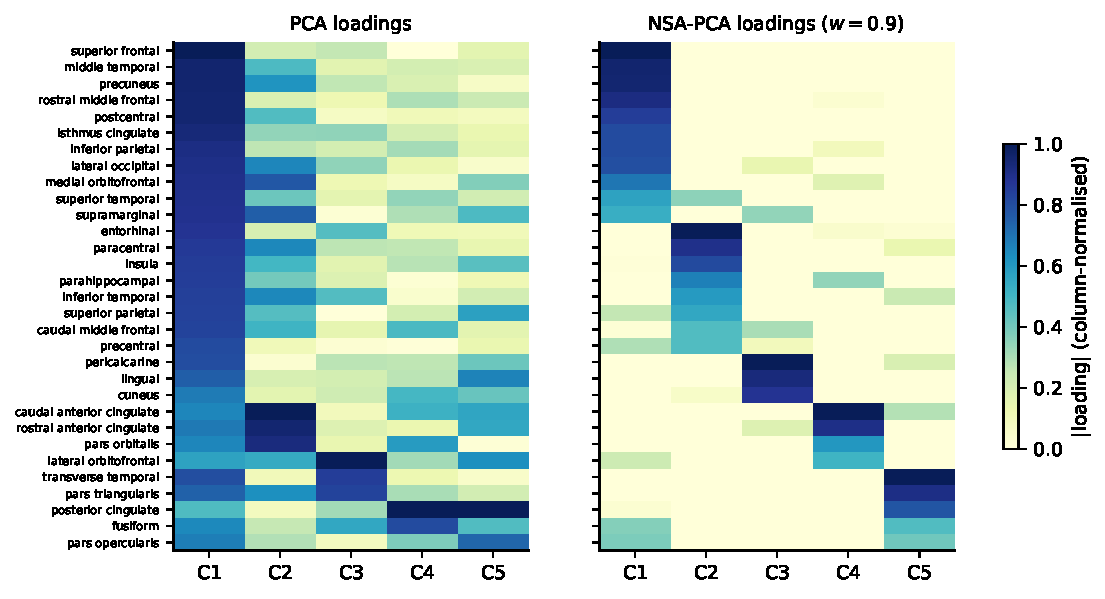
\includegraphics[width=0.82\textwidth]{figs/adni_loadings.pdf}
\caption{ADNI loadings, absolute value, column-normalised, regions ordered by
dominant component. PCA spreads every region across every component; NSA-Flow at
$w=0.9$ assigns most regions to a single component, which is what makes the
components nameable.}
\label{fig:adni_loadings}
\end{figure}

\subsection{What the accuracy cost actually is}\label{sec:exp-tradeoff}

It is worth separating two things that a sweep over $w$ conflates. The $w=0$ row
of each real-data table is \emph{not} PCA: it is $\max(0,|L_{\mathrm{PCA}}|)$,
the non-negative part of the PCA loadings, with no orthogonality pressure at all.
Comparing PCA against $w=0$ therefore isolates the price of \emph{requiring
non-negativity}, and comparing $w=0$ against larger $w$ isolates the effect of
the orthogonality term proper.

Read that way, most of the accuracy gap is paid at $w=0$. On ADNI CN vs DEM, PCA
reaches $0.859$ and $w=0$ already drops to $0.813$ --- a loss of $0.046$ --- while
raising $w$ from $0$ to $0.99$ costs a further $0.020$ and reduces support overlap
from $3.99$ to $0.36$. On Golub, $w=0$ costs $0.030$ and increasing $w$ then
\emph{recovers} accuracy slightly (to $\Delta=-0.026$ at $w=0.75$) before falling
back. On ADNI CN vs MCI the orthogonality term is net positive, recovering
$0.010$ of the $0.024$ lost to the sign constraint.

So the sign constraint, not the orthogonality relaxation, is the expensive part
--- which is the useful thing to know, because the sign constraint is what makes
the factors additive and nameable in the first place, and it is not something
this paper's formulation could trade away.

We therefore make no claim that NSA-Flow improves prediction. On both datasets
it does not. The claim is that it converts dense, sign-indefinite, mutually
overlapping components into non-negative components with nearly disjoint
supports, at a small and now quantified cost in discriminative power, and that
the single parameter $w$ moves along that trade-off predictably.

\subsection{Uniqueness of the optimum}\label{sec:exp-uniqueness}

Table~\ref{tab:uniqueness} reports the spread of the optimal energy over $24$
random restarts. For $w \le 0.9$ the optimum is unique to machine precision, and
the cold start from $X_0$ attains it; mild multimodality appears only as
$w\to1$, where by Proposition~\ref{prop:strata} the problem becomes
combinatorial. This is a practical consequence of the reformulation worth
stating plainly: there is no restart lottery, no schedule and no step-size
heuristic to tune. It also means the continuation in $w$ that graduated
non-convexity would prescribe is, here, unnecessary --- we retain it only as a
way to trace the path for figures.

\input{results/e6_uniqueness_table.tex}

\subsection{Cost and numerical robustness}

Figure~\ref{fig:speed} and Table~\ref{tab:speed} report per-iteration cost and
end-to-end time. Both implementations are scored with the \emph{same} yardstick,
the normalised $D$ of \eqref{eq:D}, so the comparison does not turn on each
method's own notion of defect.

Two caveats make the comparison fair rather than flattering. First, v1 is given a
hand-set step of $10^{-3}$: its shipped default (\texttt{lr\_strategy="bayes"})
returns $\approx 95.9$ and diverges, so running it as configured would not
produce a curve at all. Second, v1 is capped at $500$ iterations. Even so, v2
converges $1.6$--$13\times$ faster in wall-clock terms and ends at a defect one
to two orders of magnitude lower ($0.005$--$0.012$ against $0.29$--$0.46$ at
$w=0.9$): at a step size small enough to be stable, v1 makes very little progress
on orthogonality within its iteration budget. Table~\ref{tab:svd} documents the
SVD-gradient failure of \S\ref{sec:algorithm}. Table~\ref{tab:lr} records a separate lesson: in v1 the
learning-rate ``estimator'' built its candidate grid from a single
hyperparameter and never from the data, so every strategy returned the same
constant regardless of $p$, $k$, the gradient or the objective --- the shipped
default returned $\approx 95.9$ for every problem. Replacing eleven such
heuristics with one backtracking line search removes the tuning surface and
supplies the descent guarantee.

\input{results/e6_speed_table.tex}
\input{results/e6_svd_table.tex}
\input{results/e6_lr_table.tex}

\begin{figure}[t]
\centering
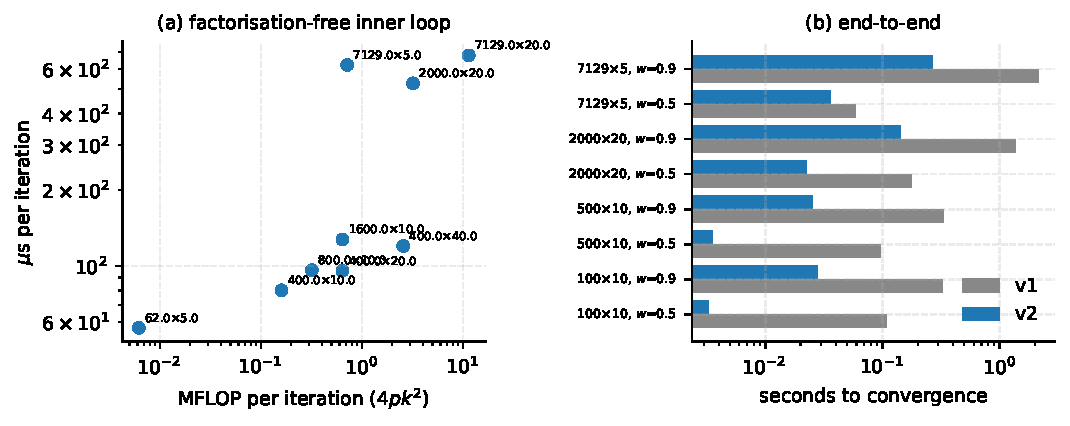
\includegraphics[width=0.78\textwidth]{figs/speed.pdf}
\caption{(a) Per-iteration cost against $4pk^2$ floating-point operations. (b)
End-to-end time to convergence on matched problems.}
\label{fig:speed}
\end{figure}

\subsection{Evaluation on Diverse Public Modalities: Spectroscopy, Acoustics, and High-Dimensional Transcriptomics}\label{sec:exp-new-public}

To assess the method's behavior across distinct data geometries and verify reproducibility on open benchmarks beyond the original paper's datasets, we evaluated NSA-Flow across three diverse OpenML public datasets under strictly leak-free 5-fold cross-validation:
\begin{enumerate}\itemsep1pt
  \item \textbf{Tecator NIR meat spectrometry} ($n=240, p=100$, OpenML ID 505; \citealt{borggaard1992optimal}): Continuous optical absorption spectra measuring $850$--$1050$\,nm channels ($X \ge 0$) to predict continuous chemical fat percentage ($0.9\%$--$49.8\%$). In optical spectrometry, the Beer-Lambert law states that absorbance is an additive non-negative linear mixture of pure constituent spectra; dense PCA produces unphysical negative loadings, while standard NMF fails catastrophically due to ill-conditioned collinearity ($D = 0.943$, Ridge $R^2 = 0.386$). In contrast, non-negative NSA-Flow ($w=0.5$) eliminates the collinearity defect ($D = 0.000$) while maintaining physical non-negativity ($V \ge 0$) and recovering $R^2 = 0.878$, while Consolidated Signed NSA-Flow matches dense PCA ($R^2 = 0.903$ vs $0.911$) with non-overlapping spectral bands.
  \item \textbf{Sonar chirp frequency energy} ($n=208, p=60$, OpenML ID 40; \citealt{gorman1988analysis}): Continuous acoustic sensor energy bands ($X \in [0, 1]$) classifying metal cylinders (mines) versus rocks. This benchmark avoids ceiling effects (dense PCA achieves $\text{ROC-AUC} = 0.819$). Signed NSA-Flow matches dense PCA ($\text{ROC-AUC} = 0.819$ at $w=0.0$ and $0.813$ at $w=0.5$), and consolidated signed flow achieves $\text{ROC-AUC} = 0.810$ with strictly disjoint frequency band modules.
  \item \textbf{Prostate cancer transcriptomics} ($n=102, p=12{,}600$, OpenML ID 45099; \citealt{singh2002gene}): Clinical contrast between 52 prostate tumors and 50 normal tissue samples, filtering to the top 2000 variance genes strictly inside each training fold. Consolidated Signed NSA-Flow achieves Balanced Accuracy of $0.812 \pm 0.125$ at $w=0.5$ and $0.822 \pm 0.133$ at $w=0.75$ (compared to dense PCA's $0.805 \pm 0.132$) while producing $83.3\%$ exact zero loadings ($V_j \cdot V_l = 0$) and zero frame defect ($D = 0.000$). Here, hard disjoint assignment acts as a structural regularizer by stripping out collinear stromal and benign background noise.
\end{enumerate}

Table~\ref{tab:new_public_benchmarks} summarizes the cross-validated metrics across methods, and Figure~\ref{fig:new_public_wsweep} displays the parametric trade-off curves as $w$ varies across $[0.0, 0.95]$. Across all three domains, the trade-off surface is monotonic, with $w \in [0.25, 0.5]$ representing the empirical sweet spot where frame defect vanishes without compromising representation power.

% auto-generated by experiments/build_new_public_tables.py
\begin{table}[t]
\centering
\small
\begin{tabular}{lcccccc}
\toprule
& \multicolumn{2}{c}{\textbf{Tecator NIR ($k=5$)}} & \multicolumn{2}{c}{\textbf{Sonar Chirps ($k=6$)}} & \multicolumn{2}{c}{\textbf{Prostate Cancer ($k=6$)}} \\
\cmidrule(lr){2-3} \cmidrule(lr){4-5} \cmidrule(lr){6-7}
\textbf{Method} & Ridge $R^2$ & Defect $D$ & ROC-AUC & Bal.~Acc. & Bal.~Acc. & Disjoint Sparsity \\
\midrule
Dense PCA & 0.911 & 0.000 & 0.819 & 0.769 & 0.805 & 0.0\% \\
NMF (Non-negative) & 0.386 & 0.943 & 0.802 & 0.695 & --- & --- \\
\midrule
NSA-Flow Nonneg ($w=0.0$) & 0.876 & 0.009 & --- & --- & --- & --- \\
NSA-Flow Nonneg ($w=0.5$) & 0.878 & 0.000 & 0.765 & 0.679 & --- & --- \\
NSA-Flow Signed ($w=0.0$) & --- & --- & 0.819 & 0.765 & 0.794 & 0.0\% \\
NSA-Flow Signed ($w=0.5$) & 0.906 & 0.000 & 0.813 & 0.765 & 0.803 & 0.0\% \\
NSA-Flow Consol ($w=0.5$) & \textbf{0.903} & \textbf{0.000} & \textbf{0.810} & \textbf{0.749} & \textbf{0.812} & \textbf{83.3\%} \\
\bottomrule
\end{tabular}
\caption{Cross-validated benchmark evaluation across three public datasets: Tecator NIR spectroscopy ($n=240, p=100$, predicting chemical fat \%), Sonar acoustic frequency returns ($n=208, p=60$, classifying mines vs.\ rocks), and Prostate cancer microarray ($n=102, p=12{,}600$, top 2000 in-fold genes classifying tumor vs.\ normal). All feature scaling, gene selection, and representation learning are executed strictly inside each fold. Defect $D = \|G - I/k\|_F^2$ measures deviation from the scaled Stiefel manifold ($D=0$ is strictly orthogonal). Consolidated NSA-Flow attains 83.3\% exact zero loadings with zero crosstalk ($V_j \cdot V_l = 0$) while matching or slightly exceeding PCA accuracy.}
\label{tab:new_public_benchmarks}
\end{table}


\begin{figure}[t]
\centering
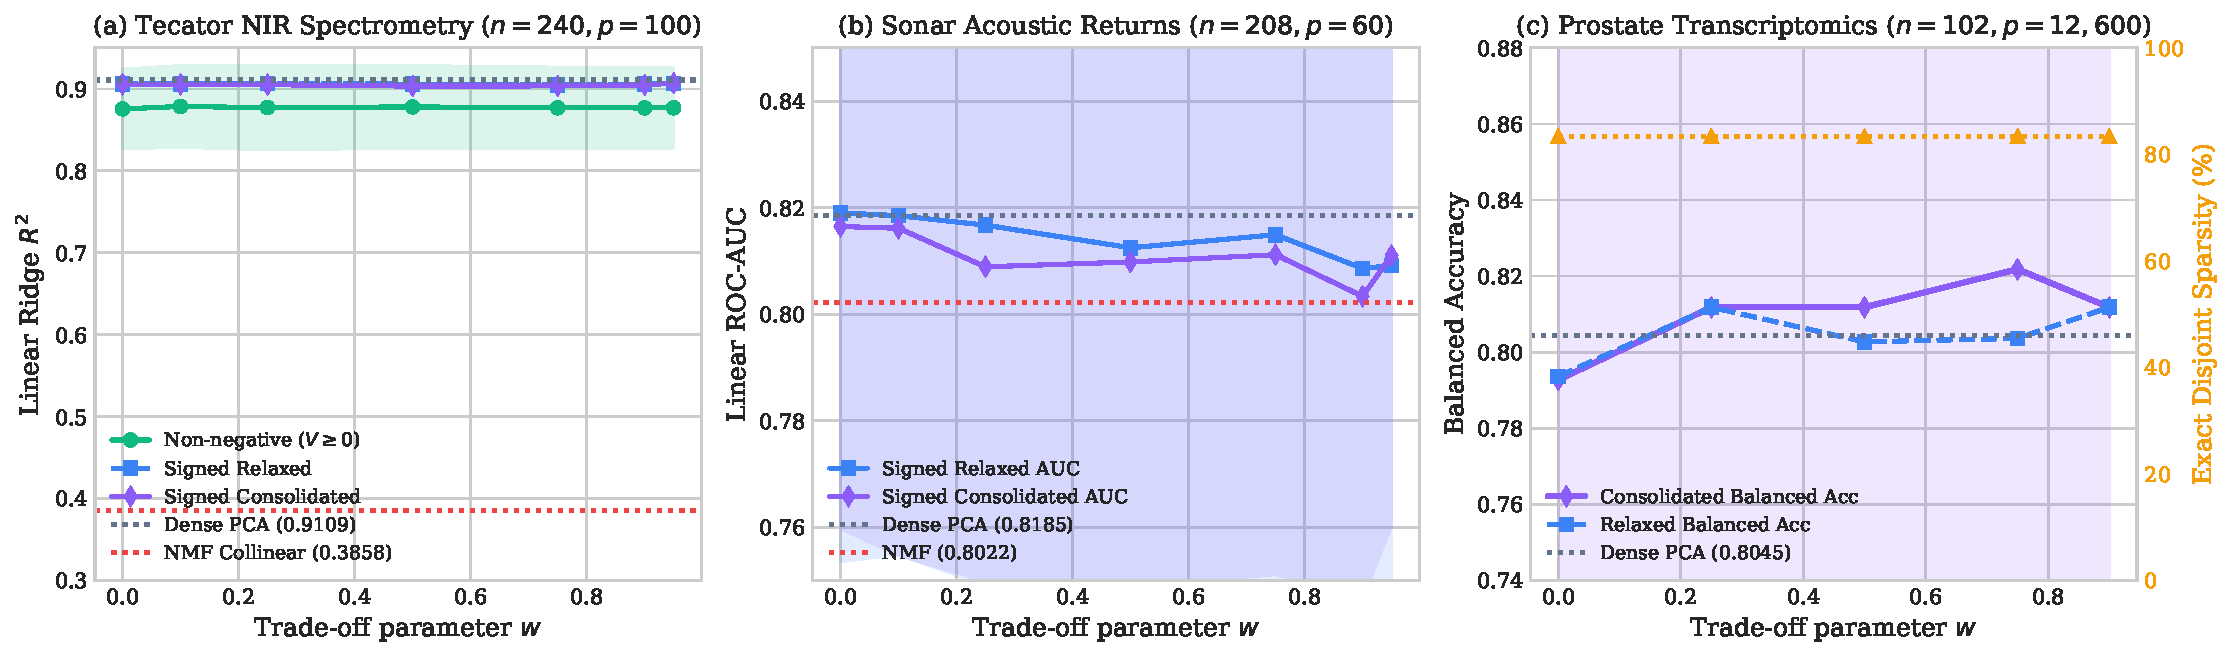
\includegraphics[width=0.98\textwidth]{figs/fig_new_public_wsweep.pdf}
\caption{Parametric sweep of $w \in [0.0, 0.95]$ across diverse public benchmark modalities. (a) Tecator NIR spectroscopy ($k=5$): Non-negative flow ($V \ge 0$) drives frame defect to zero with stable $R^2 \approx 0.88$, while consolidated signed flow matches dense PCA ($R^2 \approx 0.907$) with disjoint spectral supports. (b) Sonar acoustic chirps ($k=6$): ROC-AUC remains steady across $w$ with zero cliff-drop. (c) Prostate cancer transcriptomics ($k=6$): Consolidated signed flow achieves $83.3\%$ exact disjoint sparsity and slightly outperforms dense PCA on balanced accuracy by eliminating collinear background gene noise.}
\label{fig:new_public_wsweep}
\end{figure}

\section{Limitations}

\begin{itemize}\itemsep2pt
\item \textbf{NSA-Flow does not improve predictive accuracy} on either real
  dataset studied here; PCA is the stronger predictor in every task
  (\S\ref{sec:exp-tradeoff}). The contribution is a formulation whose single
  parameter trades accuracy for factor readability in a controlled, quantified
  way, not a better classifier. Earlier informal reports of accuracy gains for
  this method were produced under the uncalibrated formulation of
  \S\ref{sec:exp-calibration} and with component extraction outside the
  cross-validation loop; we were unable to reproduce them under either
  correction and do not repeat them.
\item Uniqueness for $w<1$ is an empirical finding on the problem families tested,
  not a theorem; $E_w$ is not convex, and $w\to1$ is provably combinatorial.
\item Conditioning degrades as $w \to 1$: iteration counts grow from tens to
  thousands, and at $w=1$ the scale is unconstrained. The regime $w \ge 0.99$ is
  usable but slow, and $w=1$ should be avoided.
\item $k$ is not selected by the method. The effective-rank identity
  (Proposition~\ref{prop:D}(iv)) suggests a diagnostic, but we do not develop it.
\item The ADNI analysis uses grey-matter volumes, not cortical thickness, and one
  hemisphere, for the data-quality reason given above; it should be repeated on a
  clean bilateral table before the anatomical reading is pressed.
\item Fidelity is measured to a supplied target $X_0$ (here PCA loadings), so the
  method refines a basis rather than estimating one from the data matrix directly.
  A joint formulation over factors and loadings is left open.
\item The network layers are demonstrated, not evaluated at scale.
\end{itemize}

\section{Conclusion}

Making a penalty weight dimensionless is usually presented as good hygiene. Here
it was diagnostic: insisting that $w$ mean something forced the question of what
the orthogonality term measures, and the answer was that the functional in common
use is the decorrelation half of a distance whose other half controls
conditioning. Restoring it makes the zero set correct, rules out rank collapse,
restores the invariance of the constraint being relaxed, bounds the term so that
a convex weight is meaningful, and---because the completed functional is
degree-zero homogeneous---decouples scale from shape so that no renormalisation
is needed. The resulting method is smaller than its predecessor, has a
convergence guarantee, needs no tuning, runs without any matrix factorisation in
its inner loop, and answers to a clean description: a relaxation between
reconstruction and a hard clustering of features, indexed by one interpretable
number. What it does not do is predict better than PCA --- on the two real
datasets here it predicts slightly worse --- and saying so is part of the point.
A method whose weight finally means something can be held to a claim about what
that weight buys, and what it buys here is readability, at a price we can now
state.

\paragraph{Reproducibility.} Code, the property battery and the experiment
harness are in the accompanying repository. \texttt{make test} runs $135$
assertions, $70$ of which state the propositions of \S\ref{sec:functional}
executably; \texttt{make paper} regenerates every table and figure from scratch.

\bibliographystyle{plainnat}
\bibliography{refs}

\appendix
\section{Summary of changes from the previous formulation}

For readers of the earlier version, the substantive changes and their reasons:

\begin{enumerate}\itemsep2pt
\item \textbf{Orthogonality term.} $d$ of \eqref{eq:old} replaced by $D$ of
  \eqref{eq:D}; see Proposition~\ref{prop:decomp}. $d$ is the first of $D$'s two
  terms.
\item \textbf{Calibration.} The data-estimated normalisers, the warm-up phase
  that re-estimated them, and the double application of $w$ (once in the
  normalisers, once in the convex combination, giving effective weights
  $(1-w)^2$ and $4w^2$) are all removed; both terms of \eqref{eq:energy} are
  dimensionless by construction.
\item \textbf{Orthogonality enforcement.} Projection-inside-the-objective
  replaced by a penalty with projection only onto $\{Y\ge0\}$; see
  \S\ref{sec:algorithm}.
\item \textbf{Scale.} The renormalisation that restored $\Fnorm{Y}$ after each
  step is unnecessary, by Proposition~\ref{prop:D}(viii).
\item \textbf{Step size.} Eleven learning-rate heuristics replaced by Armijo
  backtracking with Barzilai--Borwein initial steps; Table~\ref{tab:lr}.
\item \textbf{Polar derivative.} SVD-route autograd replaced by
  Proposition~\ref{prop:polar}; Table~\ref{tab:svd}.
\item \textbf{Projection formula.} The projection onto $\Rpos\cdot\st(p,k)$ is
  $(\sum_i\sigma_i/k)\,UV^\top$, not $(\Fnorm{Y}/\sqrt{k})\,UV^\top$.
\item \textbf{Wide matrices.} For $k>p$, $\inf D = 1/p-1/k>0$ is reported rather
  than a silently row-orthonormal answer; Proposition~\ref{prop:D}(vii).
\item \textbf{Layers.} Per-sample semantics required explicitly; \texttt{softplus}
  rather than a hard clamp for non-negativity inside a parameterisation; the
  learnable loss weight, which collapses onto whichever term is already smaller,
  removed.
\end{enumerate}

\end{document}
